
\section{Empirical results for BO and VC data}
\label{sec:empirical_results_bovc}


Following the conclusions from the simulation study, we use the Preqin data from Section \ref{sec:data} and form vintage-year portfolios (VYPs) to estimate simple linear SDF models for the Buyout (BO) and Venture Capital (VC) sub-samples individually.
For each model specification, we report asymptotic standard errors (SE$_A$) from the SHAC framework alongside $hv$-block cross-validation fold dispersions (SD$_{CV}$), defined as the standard deviation of parameter estimates across hold-out folds.
We analyze BO and VC as two distinct asset classes with fundamentally different risk profiles and report both equal-weighted (EW) and value-weighted (FW) estimates across a grid of compounding Horizons.
Throughout this section, $t_A$ denotes the $t$-ratio based on asymptotic standard errors; $\mathrm{SR}_{CV}$ (stability ratio) denotes the ratio of the full-sample estimate to the cross-validation fold dispersion, i.e., $\mathrm{SR}_{CV} := \hat{\theta} / \mathrm{SD}_{CV}$\footnote{All R code and data are available in an online repository: \url{https://github.com/quant-unit/Fundwise_SDF/tree/master/r_project}.}.
As emphasized in Remark~\ref{rem:cv_diagnostic}, $\mathrm{SR}_{CV}$ is a stability diagnostic and should not be interpreted as a test statistic with a known null distribution.

\paragraph{Summary BO data.}
The Buyout (BO) sample contains 1450 distinct funds spreading over 36 vintage years.
The vintage year distribution is as follows: 1985 (2), 1986 (3), 1987 (5), 1988 (6), 1990 (2), 1991 (3), 1992 (6), 1993 (5), 1994 (16), 1995 (13), 1996 (15), 1997 (18), 1998 (45), 1999 (31), 2000 (42), 2001 (27), 2002 (21), 2003 (30), 2004 (35), 2005 (69), 2006 (83), 2007 (85), 2008 (75), 2009 (34), 2010 (44), 2011 (55), 2012 (60), 2013 (61), 2014 (72), 2015 (72), 2016 (91), 2017 (62), 2018 (72), 2019 (94), 2020 (57), 2021 (38).
The region distribution is as follows: Africa (7), Asia (42), Australasia (32), Europe (353), Latin America \& Caribbean (22), Middle East (7), North America (986).
The strategy distribution is as follows: Buyout (1449).

\begin{figure}[ht]
	\centering
	
\includegraphics[width=0.9\textwidth]{empirical/cumcashflowsBO.pdf}
	\caption{\textbf{Cumulative cash flows:} J-curves by vintage year for BO funds in Preqin dataset scaled by fund commitment. To reduce the reliance on large unrealized NAVs, vintage years younger than 2010 are excluded (green lines).}
	\label{fig:preqin_cashflows_bo}
\end{figure}

\paragraph{Summary VC data.}
The Venture Capital (VC) sample contains 1241 distinct funds spreading over 38 vintage years.
The vintage year distribution is as follows: 1982 (1), 1985 (4), 1986 (4), 1987 (2), 1988 (1), 1989 (1), 1990 (7), 1991 (3), 1992 (7), 1993 (6), 1994 (6), 1995 (8), 1996 (15), 1997 (16), 1998 (30), 1999 (45), 2000 (79), 2001 (50), 2002 (36), 2003 (20), 2004 (38), 2005 (43), 2006 (51), 2007 (66), 2008 (57), 2009 (25), 2010 (27), 2011 (34), 2012 (34), 2013 (39), 2014 (40), 2015 (50), 2016 (52), 2017 (70), 2018 (65), 2019 (84), 2020 (68), 2021 (56).
The region distribution is as follows: Africa (2), Asia (54), Australasia (10), Europe (150), Latin America \& Caribbean (3), Middle East (29), North America (992).
The strategy distribution is as follows: Early Stage (348), Early Stage: Seed (66), Early Stage: Start-up (42), Expansion / Late Stage (153), Venture (General) (600), Venture Debt (31).

\begin{figure}[ht]
	\centering
	
\includegraphics[width=0.9\textwidth]{empirical/cumcashflowsVC.pdf}
	\caption{\textbf{Cumulative cash flows:} J-curves by vintage year for VC funds in Preqin dataset scaled by fund commitment. To reduce the reliance on large unrealized NAVs, vintage years younger than 2010 are excluded (green lines).}
	\label{fig:preqin_cashflows_vc}
\end{figure}


\subsection{The impact of unseasoned funds and reported NAVs}
\label{sec:empirical_vintage_cutoffs_bovc}

Figure~\ref{fig:max_vintage_BOVC_MKT} presents the vintage-year cutoff sensitivity analysis separately for BO and VC (an analogous analysis for aggregate PE is reported in Appendix~\ref{sec:empirical_vintage_cutoffs}).
The same upward-drift pattern documented for PE is clearly present in both sub-samples: as more recent, unseasoned vintages are included, the estimated market beta increases monotonically.
For BO under equal weighting, $\hat{\beta}_{\mathrm{MKT}}$ rises from approximately 0.87 with a 2011 vintage cutoff to roughly 1.05 with the full sample (2021); the value-weighted estimates show an analogous but slightly more pronounced increase.
For VC, the drift is even more severe in absolute terms due to the higher baseline beta: the EW estimate climbs from approximately 1.35 (2011 cutoff) through 1.85 with the full sample.
As with PE, discounting all final NAVs by 50\% eliminates the upward trend and confirms that the drift is attributable to the outsized mechanical reliance on subjectively reported Net Asset Values for young funds.
These findings reinforce the sample restriction to the 2010 maximum vintage year applied throughout the remainder of this section.

\begin{figure}[htbp]
	\centering
	\begin{minipage}{0.5\textwidth}
		\centering
		
\includegraphics[width=0.9\textwidth]{empirical_bovc/max_vintage_BO_MKT_combined_NC}
	\end{minipage}\hfill
	\begin{minipage}{0.5\textwidth}
		\centering
		
\includegraphics[width=0.9\textwidth]{empirical_bovc/max_vintage_VC_MKT_combined_NC}
	\end{minipage}
	\caption{\textbf{Sensitivity analysis ($MKT$ factor):} Single-factor model for BO (left) and VC (right) using VYP with different vintage-year cutoffs (asymptotic estimates). For each asset class, the two left charts show the standard baseline (full NAV as final cash flow), while the two right charts apply a 50\% discount to all final NAVs.}
	\label{fig:max_vintage_BOVC_MKT}
\end{figure}


\subsection{Single market-factor models}
\label{sec:empirical_single_bovc}

Tables~\ref{tab:empirical_bo_mkt}--\ref{tab:empirical_vc_mkt} and Figure~\ref{fig:empirical_BOVC_MKT} report the single-factor MKT model for BO and VC across Horizons from 0 to 30 years.
As expected from the broader PE results, the market beta declines with the compounding Horizon for both asset classes.

For BO, the estimates are close to their PE counterparts: under EW, $\hat{\beta}_{\mathrm{MKT}}$ ranges from approximately 1.19--1.23 at short Horizons (0--5~years) and decreases to 0.62 at 25--30~years; under FW, the corresponding range is 1.15--1.19 down to 0.60.
The divergence between asymptotic and cross-validation diagnostics persists: asymptotic $t$-ratios ($t_A$) are moderate at short Horizons (e.g., 1.59 under EW at 0~years) and decline further at longer Horizons, while the cross-validation stability ratios remain high throughout ($\mathrm{SR}_{CV}$ ranging from 4.38 to 11.46 under EW and from 2.67 to 7.14 under FW), indicating robust stability across data subsets.

For VC, the market beta is substantially higher across all Horizons, consistent with venture capital's greater sensitivity to systematic risk.
Under EW, $\hat{\beta}_{\mathrm{MKT}}$ reaches approximately 1.95--2.00 at 2.5--5~years and converges toward 1.01--1.14 beyond 25~years; under FW, the corresponding range is 1.69--1.70 down to 0.79--0.88.
Despite the higher parameter variability reflected in larger asymptotic standard errors (SE$_A$ of 1.2--1.8), the cross-validation stability diagnostics indicate robust estimates ($\mathrm{SR}_{CV}$ of 3.52--4.49 under EW; 3.20--6.72 under FW), although somewhat lower than the BO stability ratios due to the more heterogeneous VC fund universe.
The converged long-horizon estimates (BO $\approx 0.62$, VC $\approx 1.0$--$1.1$ under EW) are economically plausible: BO funds, which invest in mature companies with stable cash flows, exhibit market exposure comparable to or slightly below that of broad PE, while VC funds, which back early-stage ventures with highly uncertain outcomes, retain a substantially higher beta even at seasoned Horizons.

\begin{figure}[htbp]
	\centering
	\begin{minipage}{0.5\textwidth}
		\centering
		
\includegraphics[width=0.9\textwidth]{empirical_bovc/empirical_BO_MKT}
	\end{minipage}\hfill
	\begin{minipage}{0.5\textwidth}
		\centering
		
\includegraphics[width=0.9\textwidth]{empirical_bovc/empirical_VC_MKT}
	\end{minipage}
	\caption{\textbf{Empirical ($MKT$ factor):} Single-factor model for BO (left) and VC (right) using VYP and maximum vintage year 2010.}
	\label{fig:empirical_BOVC_MKT}
\end{figure}


% Auto-generated by plot_empirical_estimates.R

\begin{table}[htbp]
	\centering
	\footnotesize
	\caption{Empirical Estimates: BO --- Single-Factor (MKT) Model}
	\label{tab:empirical_bo_mkt}
	\begin{tabular}{l *{5}{r} *{5}{r}}
		\toprule
		& \multicolumn{5}{c}{Equal-Weighted (EW)} & \multicolumn{5}{c}{Value-Weighted (FW)} \\
		\cmidrule(lr){2-6} \cmidrule(lr){7-11}
		Horizon & $\hat{\beta}$ & SE$_A$ & SD$_{CV}$ & $t_A$ & $\mathrm{SR}_{CV}$ & $\hat{\beta}$ & SE$_A$ & SD$_{CV}$ & $t_A$ & $\mathrm{SR}_{CV}$ \\
		\midrule
		0 yr & 1.225 & 0.771 & 0.113 & 1.59 & 10.59 & 1.157 & 0.990 & 0.162 & 1.17 & 6.77 \\
		0.1 yr & 1.217 & 0.769 & 0.103 & 1.58 & 11.46 & 1.146 & 0.990 & 0.153 & 1.16 & 7.14 \\
		2.5 yr & 1.190 & 0.763 & 0.125 & 1.56 & 9.35 & 1.192 & 0.991 & 0.207 & 1.20 & 5.44 \\
		5 yr & 1.188 & 0.762 & 0.136 & 1.56 & 8.58 & 1.181 & 0.991 & 0.217 & 1.19 & 5.13 \\
		10 yr & 1.010 & 0.732 & 0.163 & 1.38 & 6.19 & 0.987 & 2.389 & 0.210 & 0.41 & 4.41 \\
		12.5 yr & 0.870 & 1.793 & 0.190 & 0.48 & 4.65 & 0.879 & 2.116 & 0.219 & 0.42 & 3.77 \\
		15 yr & 0.786 & 1.601 & 0.183 & 0.49 & 4.38 & 0.799 & 1.942 & 0.215 & 0.41 & 3.45 \\
		17.5 yr & 0.713 & 2.333 & 0.157 & 0.31 & 4.65 & 0.715 & 1.954 & 0.211 & 0.37 & 3.15 \\
		20 yr & 0.651 & 2.056 & 0.116 & 0.32 & 5.70 & 0.639 & 1.823 & 0.205 & 0.35 & 2.88 \\
		22.5 yr & 0.628 & 1.967 & 0.096 & 0.32 & 6.58 & 0.608 & 1.737 & 0.206 & 0.35 & 2.71 \\
		25 yr & 0.624 & 1.955 & 0.093 & 0.32 & 6.72 & 0.603 & 1.724 & 0.207 & 0.35 & 2.67 \\
		27.5 yr & 0.624 & 1.955 & 0.093 & 0.32 & 6.72 & 0.603 & 1.724 & 0.207 & 0.35 & 2.67 \\
		30 yr & 0.624 & 1.955 & 0.093 & 0.32 & 6.72 & 0.603 & 1.724 & 0.207 & 0.35 & 2.67 \\
		\bottomrule
	\end{tabular}
	\par\vspace{2pt}
	{\scriptsize\textit{Notes:} $\hat{\beta}$ = parameter estimate; SE$_A$ = asymptotic standard error; SD$_{CV}$ = cross-validation fold dispersion (standard deviation across hold-out folds); $t_A$ = asymptotic $t$-ratio; $\mathrm{SR}_{CV}$ = stability ratio (estimate / fold dispersion). Significance markers based on $t_A$: $^{*}$\,$p<0.05$, $^{**}$\,$p<0.01$, $^{***}$\,$p<0.005$.}
\end{table}

% Auto-generated by plot_empirical_estimates.R

\begin{table}[htbp]
	\centering
	\footnotesize
	\caption{Empirical Estimates: VC --- Single-Factor (MKT) Model}
	\label{tab:empirical_vc_mkt}
	\begin{tabular}{l *{5}{r} *{5}{r}}
		\toprule
		& \multicolumn{5}{c}{Equal-Weighted (EW)} & \multicolumn{5}{c}{Value-Weighted (FW)} \\
		\cmidrule(lr){2-6} \cmidrule(lr){7-11}
		Horizon & $\hat{\beta}$ & SE$_A$ & SD$_{CV}$ & $t_A$ & $\mathrm{SR}_{CV}$ & $\hat{\beta}$ & SE$_A$ & SD$_{CV}$ & $t_A$ & $\mathrm{SR}_{CV}$ \\
		\midrule
		0 yr & 1.845 & 1.737 & 0.409 & 1.06 & 4.25 & 1.583 & 1.589 & 0.357 & 1.00 & 4.42 \\
		0.1 yr & 1.801 & 1.724 & 0.389 & 1.04 & 4.37 & 1.540 & 1.592 & 0.326 & 0.97 & 4.70 \\
		2.5 yr & 1.945 & 1.785 & 0.449 & 1.09 & 3.94 & 1.696 & 1.602 & 0.435 & 1.06 & 3.82 \\
		5 yr & 2.001 & 1.824 & 0.494 & 1.10 & 3.60 & 1.693 & 1.601 & 0.428 & 1.06 & 3.79 \\
		10 yr & 1.609 & 1.251 & 0.346 & 1.29 & 4.29 & 1.386 & 1.506 & 0.239 & 0.92 & 5.55 \\
		12.5 yr & 1.427 & 1.244 & 0.295 & 1.15 & 4.47 & 1.211 & 7.559 & 0.167 & 0.16 & 6.72 \\
		15 yr & 1.263 & 1.225 & 0.257 & 1.03 & 4.49 & 1.047 & 3.733 & 0.159 & 0.28 & 5.96 \\
		17.5 yr & 1.241 & 1.227 & 0.270 & 1.01 & 4.19 & 1.020 & 3.432 & 0.171 & 0.30 & 5.39 \\
		20 yr & 1.199 & 1.246 & 0.274 & 0.96 & 4.00 & 0.960 & 2.917 & 0.183 & 0.33 & 4.73 \\
		22.5 yr & 1.150 & 1.235 & 0.264 & 0.93 & 4.01 & 0.898 & 2.514 & 0.195 & 0.36 & 4.11 \\
		25 yr & 1.135 & 3.564 & 0.264 & 0.32 & 3.94 & 0.875 & 2.003 & 0.201 & 0.44 & 3.88 \\
		27.5 yr & 1.086 & 3.137 & 0.264 & 0.35 & 3.77 & 0.836 & 2.075 & 0.212 & 0.40 & 3.52 \\
		30 yr & 1.009 & 2.626 & 0.265 & 0.38 & 3.52 & 0.793 & 1.916 & 0.223 & 0.41 & 3.20 \\
		\bottomrule
	\end{tabular}
	\par\vspace{2pt}
	{\scriptsize\textit{Notes:} $\hat{\beta}$ = parameter estimate; SE$_A$ = asymptotic standard error; SD$_{CV}$ = cross-validation fold dispersion (standard deviation across hold-out folds); $t_A$ = asymptotic $t$-ratio; $\mathrm{SR}_{CV}$ = stability ratio (estimate / fold dispersion). Significance markers based on $t_A$: $^{*}$\,$p<0.05$, $^{**}$\,$p<0.01$, $^{***}$\,$p<0.005$.}
\end{table}


\subsection{Two-factor $\alpha+MKT$ models}
\label{sec:empirical_alpha_bovc}

Tables~\ref{tab:empirical_bo_alpha}--\ref{tab:empirical_vc_alpha} and Figure~\ref{fig:empirical_BOVC_Alpha} present the two-factor MKT~+~$\alpha$ model for BO and VC.
The results show the pathological behavior anticipated by the simulation study: once an unconstrained alpha intercept is introduced, the estimation destabilizes and the MKT loading collapses.

For BO, the alpha term absorbs the bulk of the explanatory power at short Horizons: under EW, $\hat{\alpha}$ starts at 0.009 per month and declines toward 0.002 at long Horizons, while the MKT coefficient drops to 0.14--0.38; under FW, $\hat{\alpha}$ ranges from 0.007 to 0.011 per month and the MKT loading oscillates between small positive and negative values, reaching as low as $-0.22$ at 20~years.
The asymptotic standard errors are highly erratic, with several entries at or very near zero (indicating near-degenerate regions of the objective function) interspersed with values exceeding 10.
Cross-validation fold dispersions for $\hat{\beta}_{\mathrm{MKT}}$ are large (0.30--0.52 under EW; 0.56--0.72 under FW), confirming that the collapsed point estimates are unstable across data subsets.

For VC, the two-factor model exhibits a distinctive and economically puzzling pattern.
At short Horizons (0--0.1~years under EW), the alpha term reaches its upper bound ($\hat{\alpha} = 0.020$/month) and the MKT coefficient drops to approximately 0.45, resembling the BO and PE behavior.
However, as the Horizon increases beyond 5~years, the MKT loading rises steadily to values exceeding 2.3, while the alpha estimate turns progressively negative, reaching $-0.009$/month beyond 25~years.
This reversal is unique to VC and likely reflects the extreme idiosyncratic risk inherent to early-stage ventures: at long Horizons, the optimizer increasingly attributes the high compounded returns of surviving VC funds to market co-movement rather than alpha, while the negative alpha compensates for selection effects among the funds that underperformed.
Under FW, the instability is somewhat attenuated ($\hat{\alpha}$ remains close to zero at short Horizons; $\hat{\beta}_{\mathrm{MKT}} \approx 1.69$), but the overall fragility persists, with asymptotic standard errors exceeding 6--13 across most Horizons.

The BO and VC two-factor results therefore corroborate the conclusion drawn for PE: single-factor MKT models are currently the only statistically robust specification for private equity SDF estimation given the limited cross-section of vintage-year portfolios.

\begin{figure}[htbp]
	\centering
	\begin{minipage}{0.5\textwidth}
		\centering
		
\includegraphics[width=0.9\textwidth]{empirical_bovc/empirical_BO_Alpha}
	\end{minipage}\hfill
	\begin{minipage}{0.5\textwidth}
		\centering
		
\includegraphics[width=0.9\textwidth]{empirical_bovc/empirical_VC_Alpha}
	\end{minipage}
	\caption{\textbf{Empirical ($MKT + \alpha$ model):} Two-factor model for BO (left) and VC (right) using VYP and maximum vintage year 2010.}
	\label{fig:empirical_BOVC_Alpha}
\end{figure}

% Auto-generated by plot_empirical_estimates.R

\begin{table}[htbp]
	\centering
	\footnotesize
	\caption{Empirical Estimates: BO --- MKT + Alpha Model}
	\label{tab:empirical_bo_alpha}
	\begin{tabular}{l *{5}{r} *{5}{r}}
		\toprule
		& \multicolumn{5}{c}{Equal-Weighted (EW)} & \multicolumn{5}{c}{Value-Weighted (FW)} \\
		\cmidrule(lr){2-6} \cmidrule(lr){7-11}
		Horizon & $\hat{\beta}$ & SE$_A$ & SD$_{CV}$ & $t_A$ & $\mathrm{SR}_{CV}$ & $\hat{\beta}$ & SE$_A$ & SD$_{CV}$ & $t_A$ & $\mathrm{SR}_{CV}$ \\
		\midrule
		\multicolumn{11}{l}{\textit{Panel A: Market Factor ($\beta_{MKT}$)}} \\
		\addlinespace[2pt]
		0 yr & 0.141 & 9.650 & 0.520 & 0.01 & 0.78 & -0.134 & 11.550 & 0.638 & -0.01 & -0.23 \\
		0.1 yr & 0.153 & 9.490 & 0.506 & 0.02 & 1.08 & -0.123 & 11.002 & 0.613 & -0.01 & -0.21 \\
		2.5 yr & 0.230 & 5.970 & 0.429 & 0.04 & 0.86 & -0.091 & 10.122 & 0.646 & -0.01 & -0.19 \\
		5 yr & 0.256$^{***}$ & 0.072 & 0.425 & 3.57 & 1.67 & -0.055 & 10.337 & 0.618 & -0.01 & -0.05 \\
		10 yr & 0.337 & 4.116 & 0.295 & 0.08 & 1.54 & 0.074 & 9.953 & 0.564 & 0.01 & 0.30 \\
		12.5 yr & 0.219 & 1.288 & 0.412 & 0.17 & 0.98 & -0.039 & 11.801 & 0.584 & -0.00 & 0.18 \\
		15 yr & 0.243 & 1.615 & 0.415 & 0.15 & 0.98 & -0.095 & 0.072 & 0.646 & -1.32 & 0.10 \\
		17.5 yr & 0.374 & 0.831 & 0.386 & 0.45 & 1.50 & -0.091 & 10.725 & 0.692 & -0.01 & 0.11 \\
		20 yr & 0.345 & 0.892 & 0.448 & 0.39 & 1.05 & -0.215$^{**}$ & 0.070 & 0.718 & -3.08 & 0.06 \\
		22.5 yr & 0.385 & 0.863 & 0.490 & 0.45 & 0.95 & -0.191 & 0.137 & 0.720 & -1.40 & 0.04 \\
		25 yr & 0.384 & 0.880 & 0.478 & 0.44 & 0.99 & -0.186 & 0.133 & 0.720 & -1.39 & 0.03 \\
		27.5 yr & 0.384 & 0.880 & 0.478 & 0.44 & 0.99 & -0.186 & 0.133 & 0.720 & -1.39 & 0.03 \\
		30 yr & 0.384 & 0.880 & 0.478 & 0.44 & 0.99 & -0.186 & 0.133 & 0.720 & -1.39 & 0.03 \\
		\addlinespace[4pt]
		\multicolumn{11}{l}{\textit{Panel B: Alpha ($\beta_{Alpha}$)}} \\
		\addlinespace[2pt]
		0 yr & 0.009 & 0.058 & 0.004 & 0.16 & 1.61 & 0.011 & 0.073 & 0.005 & 0.15 & 1.87 \\
		0.1 yr & 0.009 & 0.057 & 0.004 & 0.16 & 1.58 & 0.011 & 0.070 & 0.005 & 0.15 & 1.93 \\
		2.5 yr & 0.008 & 0.039 & 0.003 & 0.20 & 2.27 & 0.010 & 0.064 & 0.005 & 0.15 & 1.78 \\
		5 yr & 0.007$^{***}$ & 0.001 & 0.003 & 12.35 & 1.22 & 0.009 & 0.076 & 0.005 & 0.12 & 1.69 \\
		10 yr & 0.005 & 0.031 & 0.003 & 0.17 & 1.67 & 0.007 & 0.089 & 0.004 & 0.08 & 1.33 \\
		12.5 yr & 0.005 & 0.026 & 0.003 & 0.21 & 1.15 & 0.007 & 0.111 & 0.005 & 0.07 & 1.28 \\
		15 yr & 0.004 & 0.026 & 0.003 & 0.17 & 1.23 & 0.007$^{***}$ & 0.000 & 0.005 & 16.77 & 1.13 \\
		17.5 yr & 0.003 & 0.019 & 0.003 & 0.14 & 0.49 & 0.007 & 0.162 & 0.005 & 0.04 & 0.96 \\
		20 yr & 0.003 & 0.022 & 0.004 & 0.12 & 0.50 & 0.007$^{***}$ & 0.001 & 0.005 & 10.98 & 0.94 \\
		22.5 yr & 0.002 & 0.023 & 0.004 & 0.10 & 0.46 & 0.007$^{***}$ & 0.001 & 0.005 & 10.28 & 0.96 \\
		25 yr & 0.002 & 0.024 & 0.004 & 0.09 & 0.45 & 0.007$^{***}$ & 0.001 & 0.005 & 10.28 & 0.97 \\
		27.5 yr & 0.002 & 0.024 & 0.004 & 0.09 & 0.45 & 0.007$^{***}$ & 0.001 & 0.005 & 10.28 & 0.97 \\
		30 yr & 0.002 & 0.024 & 0.004 & 0.09 & 0.45 & 0.007$^{***}$ & 0.001 & 0.005 & 10.28 & 0.97 \\
		\bottomrule
	\end{tabular}
	\par\vspace{2pt}
	{\scriptsize\textit{Notes:} $\hat{\beta}$ = parameter estimate; SE$_A$ = asymptotic standard error; SD$_{CV}$ = cross-validation fold dispersion (standard deviation across hold-out folds); $t_A$ = asymptotic $t$-ratio; $\mathrm{SR}_{CV}$ = stability ratio (estimate / fold dispersion). Significance markers based on $t_A$: $^{*}$\,$p<0.05$, $^{**}$\,$p<0.01$, $^{***}$\,$p<0.005$.}
\end{table}



% Auto-generated by plot_empirical_estimates.R

\begin{table}[htbp]
	\centering
	\footnotesize
	\caption{Empirical Estimates: VC --- MKT + Alpha Model}
	\label{tab:empirical_vc_alpha}
	\begin{tabular}{l *{5}{r} *{5}{r}}
		\toprule
		& \multicolumn{5}{c}{Equal-Weighted (EW)} & \multicolumn{5}{c}{Value-Weighted (FW)} \\
		\cmidrule(lr){2-6} \cmidrule(lr){7-11}
		Horizon & $\hat{\beta}$ & SE$_A$ & SD$_{CV}$ & $t_A$ & $\mathrm{SR}_{CV}$ & $\hat{\beta}$ & SE$_A$ & SD$_{CV}$ & $t_A$ & $\mathrm{SR}_{CV}$ \\
		\midrule
		\multicolumn{11}{l}{\textit{Panel A: Market Factor ($\beta_{MKT}$)}} \\
		\addlinespace[2pt]
		0 yr & 0.447 & 12.644 & 0.204 & 0.04 & 3.80 & 1.688 & 12.532 & 0.555 & 0.13 & 2.49 \\
		0.1 yr & 0.411 & 15.451 & 0.223 & 0.03 & 3.35 & 1.679 & 13.262 & 0.555 & 0.13 & 2.44 \\
		2.5 yr & 1.413 & 1.965 & 0.367 & 0.72 & 3.71 & 1.561 & 5.314 & 0.293 & 0.29 & 5.39 \\
		5 yr & 1.501 & 2.041 & 0.320 & 0.74 & 4.58 & 1.507 & 5.295 & 0.258 & 0.28 & 6.14 \\
		10 yr & 1.785 & 37.591 & 0.166 & 0.05 & 10.93 & 1.898 & 22.230 & 0.124 & 0.09 & 16.03 \\
		12.5 yr & 1.981 & 3.859 & 0.173 & 0.51 & 11.48 & 2.050 & 7.583 & 0.123 & 0.27 & 17.18 \\
		15 yr & 2.142 & 12.049 & 0.436 & 0.18 & 4.56 & 2.173 & 7.354 & 0.159 & 0.30 & 13.86 \\
		17.5 yr & 2.237 & 5.334 & 0.221 & 0.42 & 10.05 & 2.218 & 6.900 & 0.195 & 0.32 & 11.51 \\
		20 yr & 2.303 & 5.077 & 0.241 & 0.45 & 9.41 & 2.238 & 6.584 & 0.236 & 0.34 & 9.53 \\
		22.5 yr & 2.324 & 4.845 & 0.248 & 0.48 & 9.15 & 2.235 & 6.482 & 0.265 & 0.34 & 8.44 \\
		25 yr & 2.327 & 4.823 & 0.247 & 0.48 & 9.21 & 2.234 & 6.501 & 0.260 & 0.34 & 8.62 \\
		27.5 yr & 2.337 & 4.778 & 0.247 & 0.49 & 9.24 & 2.242 & 6.434 & 0.252 & 0.35 & 8.92 \\
		30 yr & 2.342 & 4.726 & 0.250 & 0.50 & 9.17 & 2.245 & 6.387 & 0.253 & 0.35 & 8.91 \\
		\addlinespace[4pt]
		\multicolumn{11}{l}{\textit{Panel B: Alpha ($\beta_{Alpha}$)}} \\
		\addlinespace[2pt]
		0 yr & 0.020 & 0.077 & 0.009 & 0.26 & 1.45 & -0.001 & 0.057 & 0.010 & -0.02 & 0.45 \\
		0.1 yr & 0.020 & 0.095 & 0.009 & 0.21 & 1.43 & -0.001 & 0.060 & 0.010 & -0.02 & 0.43 \\
		2.5 yr & 0.007 & 0.010 & 0.005 & 0.73 & 1.31 & 0.001 & 0.024 & 0.003 & 0.06 & 0.59 \\
		5 yr & 0.006 & 0.010 & 0.004 & 0.58 & 1.09 & 0.002 & 0.024 & 0.003 & 0.08 & 0.32 \\
		10 yr & -0.002 & 0.174 & 0.002 & -0.01 & -1.33 & -0.004 & 0.116 & 0.001 & -0.04 & -4.05 \\
		12.5 yr & -0.005 & 0.004 & 0.001 & -1.09 & -5.23 & -0.006 & 0.012 & 0.001 & -0.54 & -6.90 \\
		15 yr & -0.007 & 0.033 & 0.002 & -0.20 & -3.01 & -0.008 & 0.043 & 0.001 & -0.18 & -7.15 \\
		17.5 yr & -0.007 & 0.032 & 0.001 & -0.24 & -9.81 & -0.008 & 0.041 & 0.001 & -0.20 & -6.28 \\
		20 yr & -0.008 & 0.030 & 0.001 & -0.27 & -9.71 & -0.009 & 0.041 & 0.002 & -0.21 & -5.59 \\
		22.5 yr & -0.008 & 0.029 & 0.001 & -0.29 & -9.19 & -0.009 & 0.041 & 0.002 & -0.21 & -5.18 \\
		25 yr & -0.009 & 0.029 & 0.001 & -0.29 & -9.40 & -0.009 & 0.041 & 0.002 & -0.21 & -5.24 \\
		27.5 yr & -0.009 & 0.029 & 0.001 & -0.30 & -9.47 & -0.009 & 0.041 & 0.002 & -0.22 & -5.46 \\
		30 yr & -0.009 & 0.029 & 0.001 & -0.30 & -9.36 & -0.009 & 0.040 & 0.002 & -0.22 & -5.51 \\
		\bottomrule
	\end{tabular}
	\par\vspace{2pt}
	{\scriptsize\textit{Notes:} $\hat{\beta}$ = parameter estimate; SE$_A$ = asymptotic standard error; SD$_{CV}$ = cross-validation fold dispersion (standard deviation across hold-out folds); $t_A$ = asymptotic $t$-ratio; $\mathrm{SR}_{CV}$ = stability ratio (estimate / fold dispersion). Significance markers based on $t_A$: $^{*}$\,$p<0.05$, $^{**}$\,$p<0.01$, $^{***}$\,$p<0.005$.}
\end{table}



\subsection{Two-factor $q^5$-factor models}
\label{sec:empirical_q_factors_bovc}

We now pair MKT with each of the four non-market $q^5$ factors (ME, IA, ROE, EG) in two-factor specifications estimated separately for BO and VC.
Because the detailed estimation tables contain extensive Horizon-by-Horizon results, we do not reproduce them here and instead summarize the key patterns visible in Figures~\ref{fig:empirical_BO_q_factors} and~\ref{fig:empirical_VC_q_factors}; the full tables are available in the accompanying online repository.

\paragraph{Buyout.}
Figure~\ref{fig:empirical_BO_q_factors} shows a uniform pattern across the four non-market factors.
At short Horizons (0--5~years), the second-factor loadings are positive and economically large: the ME loading reaches approximately 1.5--1.7 under EW (with stability ratios $\mathrm{SR}_{CV}$ of 3.2--4.1), the IA loading starts near 1.2 under EW ($\mathrm{SR}_{CV} \approx 1.5$), ROE near 0.8 ($\mathrm{SR}_{CV} \approx 1.0$), and EG near 0.6 ($\mathrm{SR}_{CV} \approx 1.4$).
As the Horizon increases, however, all four second-factor loadings decay toward zero and frequently change sign beyond 10--15~years.
The ME factor retains a moderate positive loading even at long Horizons under FW ($\hat{\beta}_{\mathrm{ME}} \approx 1.5$, $\mathrm{SR}_{CV} \approx 2.2$), but under EW the loading drops below 1.0 after 17.5~years.
The EG, IA, and ROE loadings all fluctuate around zero at intermediate and long Horizons, with cross-validation stability ratios well below conventional thresholds.
The MKT loading in these two-factor models remains similar to its single-factor counterpart (ranging from roughly 0.95 at short Horizons to 0.55--0.70 at long Horizons), showing that a second factor does not materially alter the market risk assessment.
The asymptotic standard errors are erratic throughout, often exceeding 10 and occasionally reaching triple-digit values, which highlights the unreliability of asymptotic inference in this setting.

\paragraph{Venture Capital.}
Figure~\ref{fig:empirical_VC_q_factors} displays qualitatively analogous but more extreme patterns, consistent with the higher idiosyncratic risk inherent to early-stage ventures.
At short Horizons, the second-factor loadings are strikingly large: the IA loading reaches $4.3$ under EW at the 0-year Horizon ($\mathrm{SR}_{CV} \approx 1.4$) and $4.0$ under FW, the ROE loading starts at $2.4$ (EW) and $2.0$ (FW), the EG loading at approximately $2.0$ (EW) and $2.9$ (FW), while the ME factor is the exception with a subdued loading near $0.4$--$0.5$.
All four second-factor loadings undergo dramatic sign reversals as the Horizon extends.
The IA loading, for instance, turns negative beyond 10~years and eventually reaches $-1.5$ to $-1.9$ at long Horizons with large stability ratios ($\mathrm{SR}_{CV}$ exceeding $-15$).
Similarly, EG and ROE produce large negative loadings at long Horizons ($\hat{\beta}_{\mathrm{EG}} \approx -0.9$, $\hat{\beta}_{\mathrm{ROE}} \approx -1.2$ under EW at 30~years).
These sign reversals echo the behavior documented in the simulation study (Section~\ref{sec:simulation_study}), where two-factor models exhibited severe attenuation and sign changes in the second-factor loading across Horizons.
The MKT loading in the VC two-factor models varies substantially across specifications: in the IA model it stabilizes around 1.4--1.5 at intermediate Horizons, while in the ROE and EG models it ranges from 0.5 to 2.0 depending on the Horizon and weighting scheme.

\paragraph{Summary.}
The $q^5$-factor results for BO and VC confirm the fragility of multi-factor SDF estimation documented in the preceding MKT~+~$\alpha$ analysis.
While some second-factor loadings attain statistical significance at isolated Horizons (particularly ME for BO and short-Horizon IA for VC), none of the four non-market factors produces a stable, economically interpretable loading across the full Horizon spectrum.
The pervasive sign reversals and the extreme sensitivity of point estimates to the compounding Horizon indicate that these results are driven by finite-sample noise rather than genuine systematic risk exposures.
We conclude that the $q^5$-factor two-factor models do not improve upon the single-factor MKT benchmark for either asset class.

\begin{figure}[H]
	\centering
	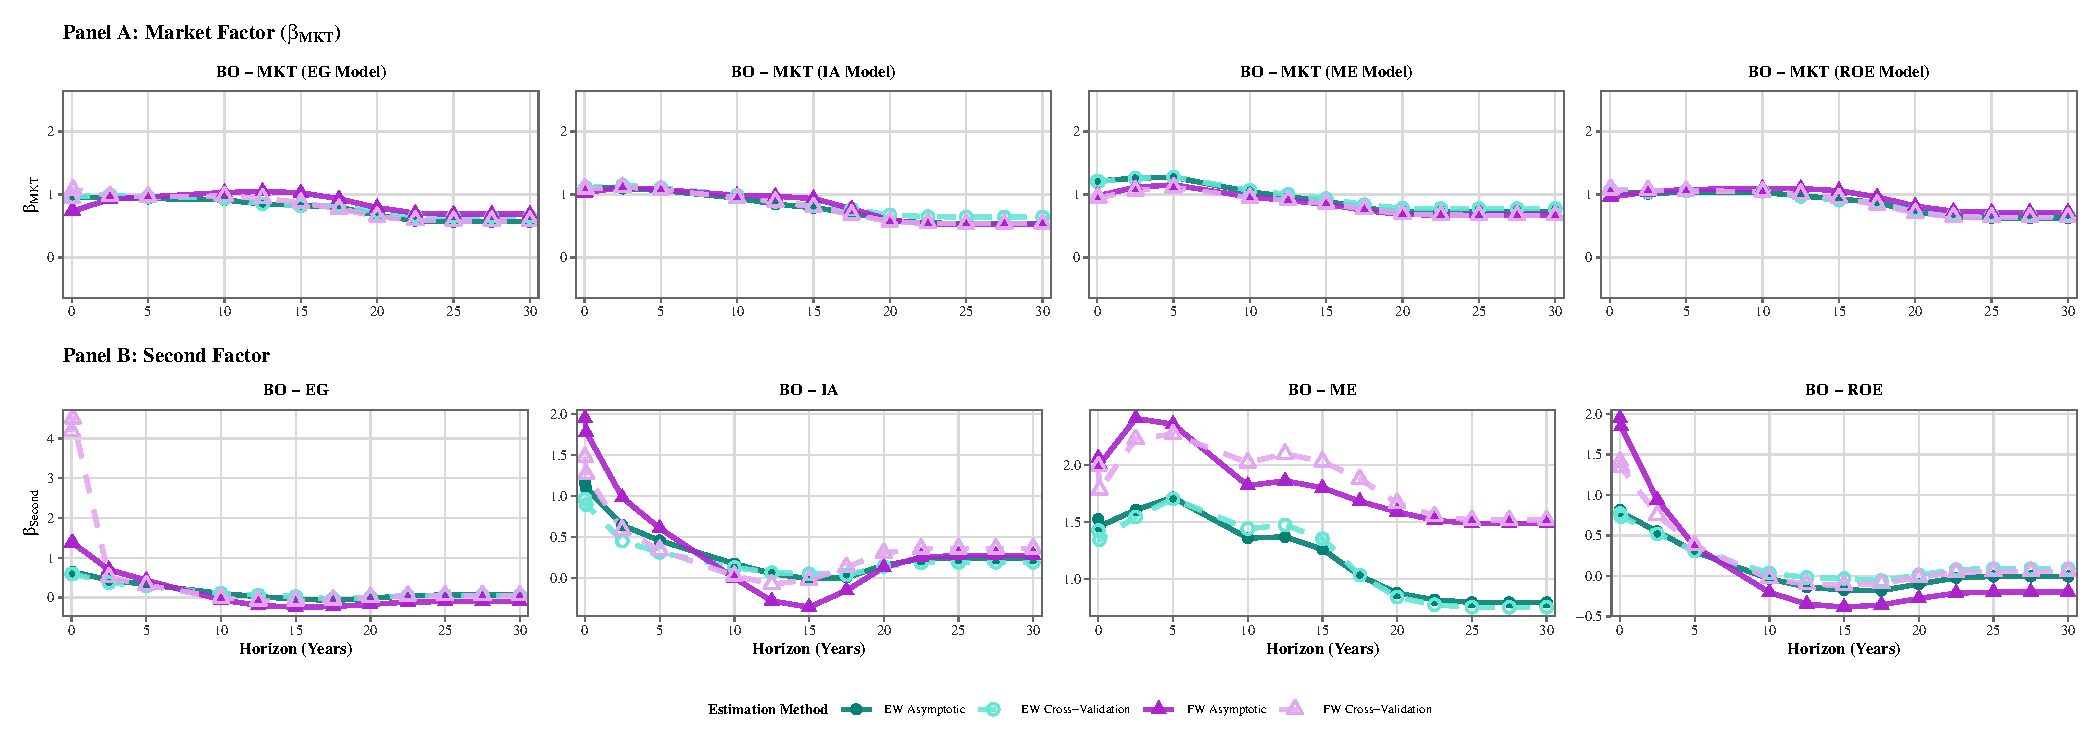
\includegraphics[width=0.9\textwidth]{empirical_bovc/empirical_BO_Multi.pdf}
	\caption{\textbf{Empirical results ($q^5$-factors):} Two-factor model for BO funds using VYP and maximum vintage year 2010.}
	\label{fig:empirical_BO_q_factors}
\end{figure}


\begin{figure}[H]
	\centering
	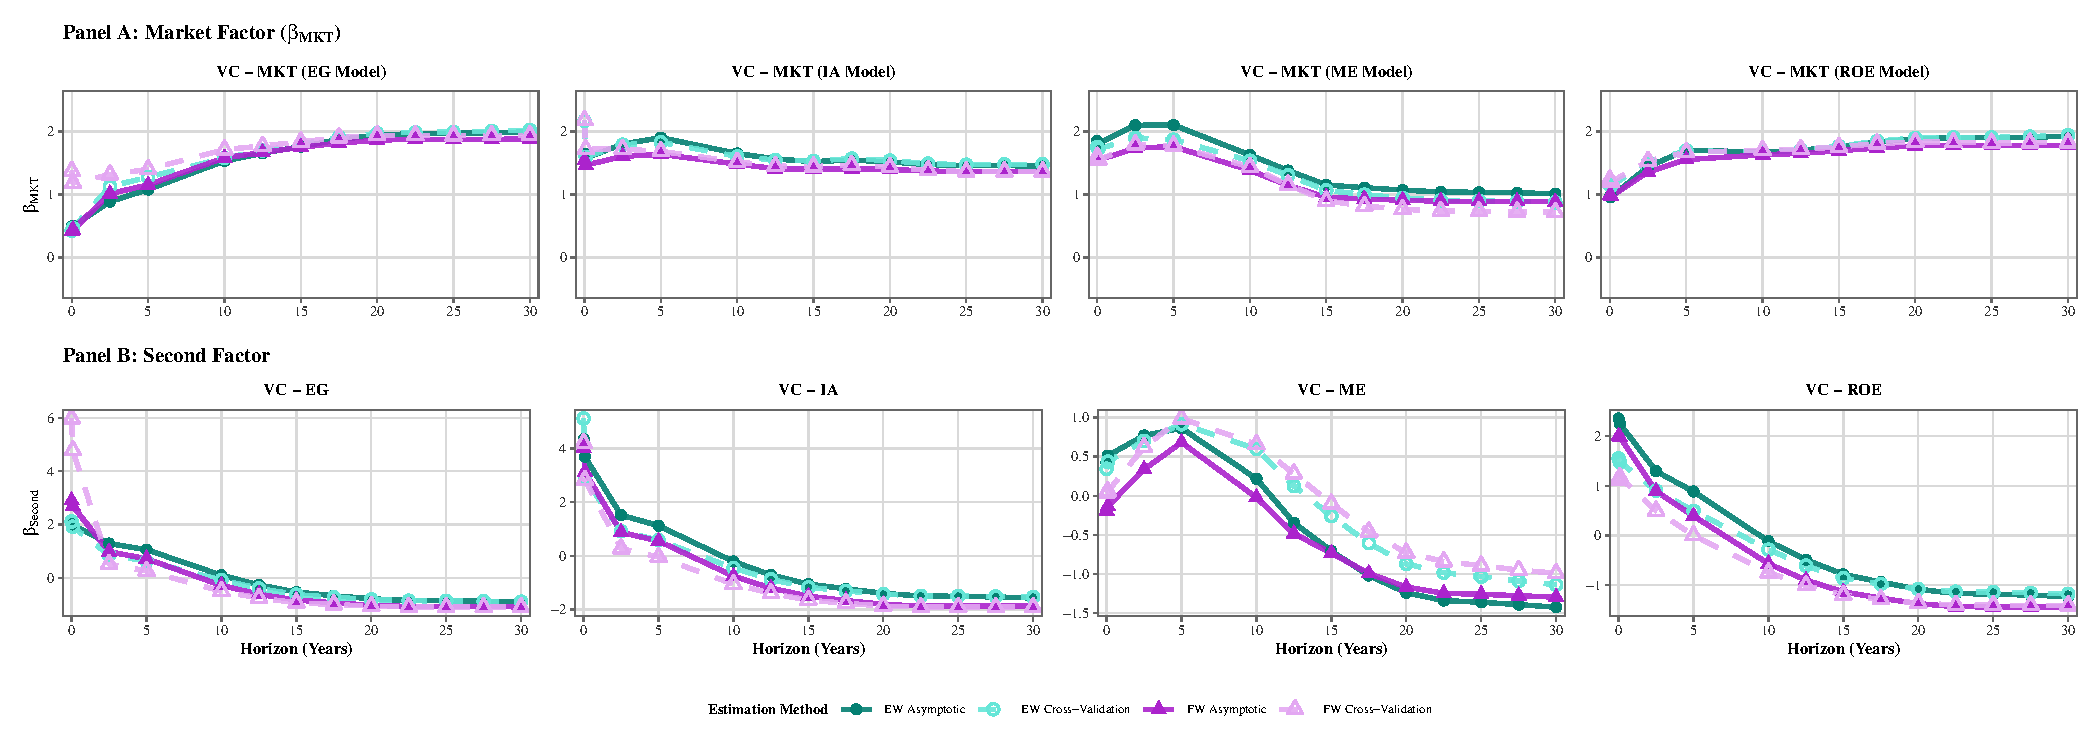
\includegraphics[width=0.9\textwidth]{empirical_bovc/empirical_VC_Multi.pdf}
	\caption{\textbf{Empirical results ($q^5$-factors):} Two-factor model for VC funds using VYP and maximum vintage year 2010.}
	\label{fig:empirical_VC_q_factors}
\end{figure}


\subsection{Interpretation}
\label{sec:empirical_interpretation}

The empirical results for Buyout and Venture Capital funds demonstrate consistent model reliability across both asset classes and weighting schemes.

\paragraph{Single-factor MKT models are the only robust specification.}
The single-factor market model produces economically plausible and statistically significant estimates for both BO and VC.
For Buyout, the market beta ranges from approximately 1.19 at the shortest Horizon to 0.62 at long Horizons under equal weighting, with cross-validation stability ratios consistently exceeding 4.0.
For Venture Capital, the corresponding range is 1.85--2.00 down to 1.01--1.14, reflecting the substantially higher systematic risk exposure of early-stage investments.
The cross-validation stability diagnostics are strong and consistent across the entire Horizon spectrum, even as asymptotic standard errors fluctuate erratically.
The divergence between asymptotic inference and cross-validation diagnostics mirrors the simulation finding that, with the limited cross-section of vintage-year portfolios, the asymptotic approximation is unreliable and overly conservative.

\paragraph{Multi-factor models are fragile.}
Both the MKT~+~$\alpha$ and the $q^5$-factor two-factor models collapse as soon as a second parameter is introduced.
In the MKT~+~$\alpha$ specification, the alpha intercept absorbs explanatory power from MKT, producing collapsed or negative market betas and erratic standard errors.
The $q^5$-factor models exhibit a pervasive pattern of sign reversals: second-factor loadings are consistently overestimated at short Horizons and attenuate toward or beyond zero at long Horizons, exactly as predicted by the simulation study in Section~\ref{sec:simulation_study}.
This fragility is not confined to a single factor or asset class; it appears across all eight specifications (four factors $\times$ two asset classes), ruling out the chance that an individual $q^5$ factor might robustly augment the market model.

\paragraph{BO--VC decomposition.}
Analyzing Buyout and Venture Capital separately provides a more informative test of model stability than reporting aggregate PE results alone.
BO and VC represent fundamentally different investment strategies: Buyout targets mature companies with leveraged balance sheets and stable cash flows, while Venture Capital finances early-stage firms with highly uncertain, option-like payoff profiles.
Despite these differences, both sub-samples exhibit the same diagnostic pattern: robust single-factor significance, alpha-induced destabilization, and second-factor fragility.
The fact that this pattern appears across two asset classes with different risk characteristics suggests that the multi-factor instability is a finite-sample identification problem, not an artifact of pooling heterogeneous fund types.

\paragraph{Reconciliation with the simulation study.}
The empirical results mirror the simulation predictions from Section~\ref{sec:simulation_study}.
First, the bias-minimizing Horizon at which the single-factor estimates stabilize (approximately 15--20~years) aligns with the 12.5--15-year optimum identified in simulation.
Second, the sign reversals and large estimation variance observed in the empirical $q^5$-factor models replicate the pathological behavior documented in the two-factor simulation experiments, where the second-factor loading underwent severe attenuation and occasionally changed sign across Horizons.
Third, the divergence between asymptotic inference and cross-validation stability diagnostics in the data is consistent with the simulation finding that asymptotic standard errors systematically overstate true parameter uncertainty in small samples.
These results show that the finite-sample challenges identified by our simulation study appear directly in empirical estimation with real-world private market data.

\paragraph{Implications for empirical practice.}
Our findings yield a clear recommendation for applied researchers and practitioners.
Semiparametric SDF estimation for private equity cash flows should be restricted to single-factor market models estimated on seasoned, vintage-year portfolios at an extended compounding Horizon of approximately 15~years.
Multi-factor models and alpha intercepts, while theoretically appealing, cannot be reliably estimated with the cross-sectional sample sizes currently available in private equity databases.
Only a substantial expansion of the available data, either through longer time series of fully seasoned funds or through larger cross-sections within each vintage year, would provide the statistical power necessary to disentangle multiple systematic risk exposures from finite-sample noise.


